\chapter{Methods}
\label{chap:methods}

Methods used in the research will be described in this chapter. In order to answer the research questions, there were two sets of experiments conducted in the study: trial and the main ones. The purpose of the trial experiments was to get an understanding of classification system potential, to test its implementation, get a better understanding of time-constrains when it comes to training and testing processes, to compare different solutions as well as to learn tools and framework used. Lessons learned during trial experiments on the limited set of images categories were further used to perform a more full study with a more broad set of categories. A bigger scale of experiments was also possible due to donated GPU by the NVIDIA Corporation for this project (see section \ref{sec:main-hw}.


\section{Metadata preparation}
\label{sec:metadata-prep}
This section describes steps that were made to process NTB images metadata in order to store it in more suitable for this project format.

NTB uses proprietary text format to store images metadata, which is called ``tfo''. These files describe such image information as date, labels, description, photographer's name etc. For the purpose of this research, only image filename, SUBJECT\_HEADING and STORAGE\_TYPE fields were used. SUBJECT\_HEADING contains a list of labels in the Norwegian language, therefore each label was translated into English using dictionary provided by NTB. 15 labels were missing translation and therefore were removed, 85 images were labeled with these tags.

Since all neural networks used in the research were designed to by trained on images with three color channels, grayscale and CMYK images were filtered out from the collection. STORAGE\_TYPE field, which among other information contain indication if the image is grayscale, was used for this purpose -- pictures which had ``svarthvitt'', ``blackandwhite'', ``monochrome'' and ``svartvit'' values in the STORAGE\_TYPE field were removed. However, it was empirically established that not all grayscale images were removed using this method, therefore, in addition, each image was read from the disk and number of its color channels was checked. The first method, therefore, was used only for optimization purposes: such images were filtered out without reading its content. From the total number of 966372 processed images, 54045 (5.59\%) were removed due to having one channel (grayscale), 2 were removed due to having four channels (CMYK) and 1 image was removed because it was missing from the image collection on the disk.

As a result of the metadata processing, a Python dictionary was built with image filenames as keys and a corresponding list of labels as values. Since this process was time-consuming (around five to six hours on PC with HDD), the resulting dictionary was saved to disk using pickle \cite{pickle} format and further read and reused in the experiments.

In addition to image metadata, the author was also provided with categories tree definition by NTB. The tree was stored in a text-based format where the parent-child relationship was indicated by TAB character. The tree was transcoded to newick \cite{newick} format by applying recursive function and further used to build in-memory tree representation via Python ETE toolkit \cite{ete3}.


\section{Trial experiment}
    The goal of the trial experiment was to get insights on a potential of the system when applied for given image collection, as well as to test implementation, training and test process, and to discover possible issues which can be addressed in the further experiments.
    
    The specialized set of experiments was used also to test the potential speedup of the training process when LMDB is used as an image data-source rather than real-time image processing.
    
    Further sections describe each part of the experiments in more details.
    
    \subsection{Selection of categories}
    The initial selection of the categories was performed based on the flat list of NTB categories, without consideration of origin tree structure. All categories were sorted by the number of images contained and all categories with less than 1000 images were dropped. Only those categories were included, which names belonged to the ``entity'' or ``sport'' classes of WordNet \cite{wordnet}. Each category in the resulting list of candidates was manually investigated and included or excluded based on the selection criteria described further.
    
    The category was excluded based on its name if:
    \begin{itemize}
        \item It was a combined term. Examples: \textit{moos-and-lichen}, \textit{museums-and-art-galleries}.
        \item It had double meaning. Examples: \textit{direction} (the sign or human pointing the direction).
        \item The term was contextual rather than visual. Examples: \textit{used-cars}, \textit{counterfeit-money}.
    \end{itemize}
    
    Random selection of images from each category was investigated and the category was included only when all criteria were met:
    \begin{itemize}
        \item All images contained entity or sport of interest and it was clearly visible
        \item All images were consistent in the interpretation of the term
    \end{itemize}
    
    After selection of the categories, some of them were merged together or renamed. The final category list is shown in Table \ref{table:trial-categories}, as well as the names of the NTB labels that were merged together to form a new category.
    
    \begin{table}[H]
    \small
    \centering
    \csvreader[
        separator=semicolon,
        tabular=|l|p{0.6\textwidth}|,
        table head=\hline \textbf{Category} & \textbf{NTB categories}\\\hline\hline,
        table foot=\hline,
        head to column names,
        late after line=\\\hline,
    ]
    {tables/trial-categories.csv}
    {}
    {\category & \ntbcategories}
    
    \caption{Trial experiment categories selection}
    \label{table:trial-categories}
    \end{table}
    
    In this way, the selected categories were subjectively more consistent in their image content and therefore potentially less challenging for an automated system to learn from.
    
    For the experiment with LMDB \cite{lmdb} used as a data source (see section \ref{sec:trial-training}), a specific set of categories was used, limited to types of skiing. For single-label cases, when there is only one label on the image, the interface for creation of LMDB entries is much simpler than for the multi-label cases. Skiing subcategories were therefore chosen since these were mutually exclusive in NTB's dataset.
    
    \subsection{Dataset preparation}
    \label{sec:trial-dataset-prep}
    The base training dataset was created using selected categories. Distribution of images for each category is shown on Figure \ref{fig:trial-distribution-base}. The chart clearly indicates a big imbalance in the number of images per category. Undersampling approach was used to solve this issue, where random images from the majority categories were removed from the dataset. There is additional challenge connected with a multi-label classification that rises when some of the categories are tightly coupled, meaning that one image can be part of several categories. In this case, by removing an image from one category, it will have to be removed from all other categories it belongs to in order to keep consistency in the dataset. If the image will not be removed from the whole dataset, it can lead to false-positive errors (which are not errors originally) during the training. The problem arise when the image will have to be removed from the category with a small number of images initially. There are two choices in this case:
    
    \begin{itemize}
        \item Remove image from all categories. In this case, it is possible to achieve state when no category has more pictures than a particular threshold, but this can lead to an even smaller number of images in underrepresented categories.
        \item Keep the image in all categories. In this case, categories with a small number of pictures will be preserved, however, it can be a situation when some categories acceded specified threshold.
    \end{itemize}
    
    \begin{figure}[h!]
        \centering
        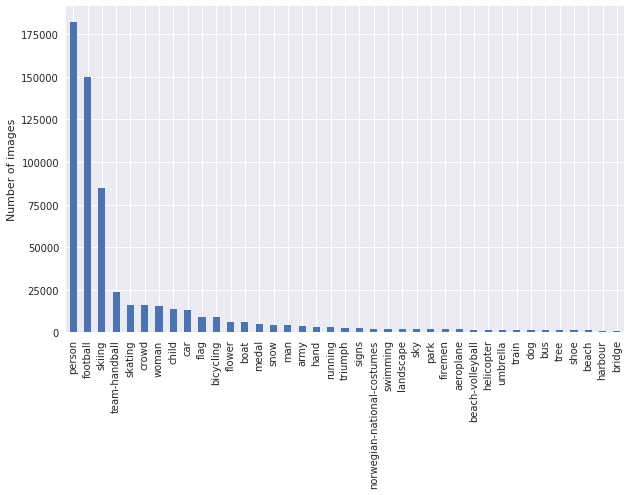
\includegraphics[width=\textwidth]{trial-distribution-base}
        \caption{Number of images per category distribution}
        \label{fig:trial-distribution-base}
    \end{figure}
    
    The decision on which choice to make depends on the particular case with the specific imbalance level, the level of intersection between categories as well as a total number of images in all categories. Since some of the categories from the constructed dataset in this research had only 1000 images, the second option of keeping images in all categories was chosen.
    
    The resulting balanced dataset with the threshold level of 10000 is shown on Figure \ref{fig:trial-distribution-balanced}. Due to the chosen threshold, \textit{person}, \textit{football}, \textit{skiing}, \textit{team-handball}, \textit{woman}, \textit{crowd}, \textit{child}, \textit{skating} and \textit{car} categories were undersampled.
    
    \begin{figure}[h!]
        \centering
        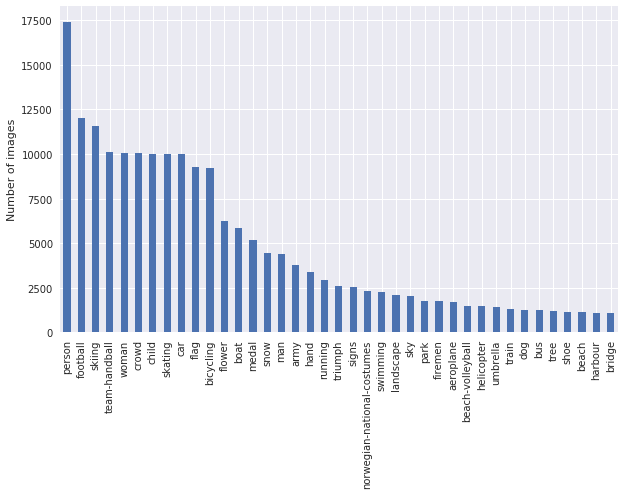
\includegraphics[width=\textwidth]{trial-distribution-balanced}
        \caption{Number of images per category distribution after balancing the dataset}
        \label{fig:trial-distribution-balanced}
    \end{figure}
    
    In order to test how dataset improvement can influence resulting system performance, additional experiment was conducted where context content was filtered-out from some of the categories. In particular, pictures labeled with \textit{portrait}, \textit{press-conferences} and \textit{coaches} were removed from all categories except \textit{woman}, \textit{umbrella}, \textit{hand}, \textit{person}, \textit{norwegian-national-costumes}, \textit{child}, \textit{medal}, \textit{triumph}, \textit{man}. The motivation was to remove such pictures that can be classified to a particular category only using additional contextual information, for example to remove press-conference pictures in the category of football.
    
    After the dataset is generated, it has to be split into three parts: training, validation, and test. The training set is used directly in the training process, validation set is used to control training process and to find the point of its termination, the test set is used in the testing process to check the resulting system performance. The intersection of all of this sets should be an empty set, meaning that each image should be part of only one of them. Having separate testing set should potentially increase the generalizability of results since in this case system will be tested on new images, the ones that were not used during the training process. 
    
    In this research, the original dataset was randomly split for each category with the ratio of 0.6, 0.2, 0.2 accordingly. For example, around 60\% of the images from the category \textit{person} were assigned to the training set, 20\% -- to the validation set and 20\% -- to the test set. The challenge on this stage is similar as to the one from the previous step -- in the case of a multi-labeling system, it is possible that some categories are tightly connected which can lead to unequally distributed images. For example, some images from the 60\% selected for the training set from the \textit{person} category can also be part of other categories, which can lead to the state when more than 60\% of images from these categories are now part of the training set. In the trial experiments, a ``priority'' algorithm of dataset split was implemented and used, where the training set had higher priority than validation and test sets, meaning that each category from the training set had a higher chance to satisfy 60\% percent requirement than ones from the other sets.
    
    The base balanced dataset, as well as training, validation and test sets, were generated randomly for each experiment. This was fixed in the main experiment in order to improve the validity of the results.
    
    \subsection{Training process}
    \label{sec:trial-training}
    Caffe \cite{Caffe} learning framework was used in the research. Specifically, pycaffe \cite{pycaffe} Python interface was used to create specification, train, and test deep neural networks.
    
    Due to the relatively old hardware available to the author during the trial experiments (see section \ref{sec:trial-hw}), CaffeNet \cite{CaffeNet} was chosen as a base neural network since it is a slightly changed version of AlexNet \cite{Krizhevsky2012ImageNetDNN} which was trained on the similar hardware.
    
    The fine-tuning approach of the pretrained network described in the section \ref{sec:transfer-learning} was used in the study. Pretrained weights for the CaffeNet were downloaded from the Caffe Model Zoo \cite{CaffeModelZoo}.
    
    Since original CaffeNet (as well as  AlexNet) was designed for single-labeling classification on ImageNet dataset, the network structure had to be adapted for the multi-labeling purpose. Specifically, Data layer, the last InnerProduct layer, and SoftMax loss layers were replaced in the model. Since Caffe Accuracy layer was not adapted to work for the multi-label case during the time of the research, it was removed from the model. The weights for the rest of the layers were copied from the pretrained model.
    
    \paragraph{Data layer}
    Caffe framework can read image data during the training process from the different sources like database, memory, or directly from files on the storage \cite{CaffeLayerCatalogue}. Due to its flexibility, Python layer was used to supply network with image data from disk, however, the additional experiment was also conducted with LMDB \cite{lmdb} as a source of data to compare the speed of training. Since CaffeNet DNN was used in the experiment, all images were resized to 227x227 and RGB channels were swapped to BGR. In a case of Python data layer, this changes were made during the training process for each image, while when LMDB was used as a datasource these transformations were performed as a separate step before training and all image data was written to a newly created LMDB file.
    
    \paragraph{InnerProduct layer}
    Since used parameters for CaffeNet were optimized to classify 1000 categories from ImageNet dataset, the last fully connected layer had to be retrained from scratch. Therefore InnerProduct layer with the name ``fc8'' which had 1000 outputs was replaced with the new one with the 39 outputs (number of selected categories).
    
    \paragraph{Loss layer}
    SoftMax loss layer used both in AlexNet and CaffeNet is only suitable for single-label classification. Therefore SigmoidCrossEntropyLoss layer was used in all experiments, which predicts the probability for each category and calculates loss:
    
    $$
    E = -\frac{1}{N} \sum_{n=1}^{N} [p_n log (\hat p_n) + (1 - p_n) log(1 - \hat p_n)]
    $$
    
    Two solver algorithms were tested in trial experiments: Stochastic gradient descent \cite{sgd} and Adam \cite{adam}. Solver hyper-parameters used for training:
    \begin{itemize}
        \item Base learning rate -- 0.0001
        \item Learning rate policy -- fixed
        \item Test iterations -- 1000
        \item momentum -- 0.9
        \item momentum2 -- 0.999
        \item delta -- $10^{-8}$
    \end{itemize}
    
    The last three parameters were used only together with Adam solver algorithm. \textit{momentum}, \textit{momentum2} and \textit{delta} parameters were set to the recommended values from the paper \cite{adam} (also default values in the Caffe framework).
    
    Even though fine-tuning approach was used in the study, all layers had the same learning rate during the training process in contrast to reducing learning rates for first layers or even freezing them completely. This was made based on the study \cite{Yosinski2014HowTransferable} were authors discovered that training all layers can give even better results compared to training only part of the layers.
    
    In order to utilize all available GPU memory as well as to improve the stability of the training, the batch size of 200 was used for training and 20 for validation. Networks for all trial experiments were trained for 1000 iterations.
    
    % caffe framework, pycaffe library, hyper parameters, fine-tuning, caffeNet
    
    % presision = N_correctly_detected_labels / N_total_detected_labels
    % recall = N_correctly_detected_labels / N_all_correct_labels
    
    % update functions (cs231 l.6):
    % * sgd -- old
    % * mu - momentum around 0.5, 0.9 or 0.99
    % * nesterov accelerated momentum (nag) even better (lookahead momentum)
    % * adagrad -- per parameter update
    % * rmsprop -- improved adagrad. Updates do not decay with time to zero
    % * adam -- rmsprop + momentum (beta1 = 0.9, beta2 = 0.995) (default one)
    
    % should decay learning rate (e.g 0.9)
    % epoch -- after seeing all images one time
    \subsection{Testing process}
    \label{sec:trial-testing}
    The ''deploy`` version of the CaffeNet was used for testing where data layer was replaced with direct Input layer and SigmoidCrossEntropyLoss replaced with the Sigmoid layer. Each image from the prepared test set was preprocessed in the same way as for training, sent as an input to a trained network and predictions for each category were obtained and stored in the numpy matrix. This matrix was then used to calculate all matrix as described further.
    
    In order to be able to compare different multi-label network implementations, \textit{Average Precision (AP)} metric was in this study, which was defined in the PASCAL Visual Object Classes Challenge \cite{Everingham2010PASCAL-VOC} in the following way:
    
    \begin{displayquote}
    For a given task and class, the precision/recall curve is computed from a method’s ranked output.Recall is defined as the proportion of all positive examples ranked above a given rank. Precision is the proportion of all examples above that rank which are from the positive class. The AP summarises the shape of the precision/recall curve, and is defined as the mean precision at a set of eleven equally spaced recall levels $[0,0.1, . . . ,1]$:
    $$
    AP = \frac{1}{11} \sum_{r \in \{0, 0.1, ..., 1\}} p_{interp}(r)
    $$
    The precision at each recall level $r$ is interpolated by taking the maximum precision measured for a method for which the corresponding recall exceeds $r$:
    $$
    p_{interp}(r) = \max_{\tilde{r}:\tilde{r} \ge r} p(\tilde{r})
    $$
    \end{displayquote}
    
    Therefore, both \textit{precision-recall curve} and \textit{average precision} were calculated for each category using numpy vectorized computations and further used for models comparison.
    
    % transformer, batches, deploy network, metrics
    \subsection{Hardware}
    \label{sec:trial-hw}
    \begin{itemize}
        \item \textbf{CPU} -- Intel Core 2 Duo
        \item \textbf{GPU} -- NVIDIA GTX 580
        \item \textbf{RAM} -- 
        \item \textbf{Storage} -- 
    \end{itemize}


\section{Main experiment}
    Lessons learning during trial experiments were used in the main set of experiments where the neural network was trained on much broader and challenging selection of categories. These experiments were also performed on the new hardware, which allowed to test more complex neural networks. Differences between two experiments are described in the following sections.
    
    \subsection{Selection of categories}
    Selection of categories for the main experiment was based on the whole NTB tree, including its structure (parent-child relationship). As a result, a new tree was created, adapted to a training of the multi-label classification system. Issues and insights discovered during this process are presented in the section \ref{sec:tree-eval}. This section describes selection criteria for categories as well as all steps taken to create the new tree.
    
    The goal of this part of the research was to create a tree of categories that would be suitable for training the multi-label image classification system, maximizing utilization of the available metadata. Therefore decisions on how to change the existing tree, which categories to include, which of them to merge into one etc were made based on:
    
    \begin{itemize}
        \item The available tree structure: the path from the root of the tree to the particular category, category children, parents, and siblings.
        \item The category name (translated from the Norwegian language as described in the section \ref{sec:metadata-prep}).
        \item The number of images in the category itself and the total number of images within all its descendants.
    \end{itemize}
    
    % All selected categories belong to one of the following WordNet categories \cite{wordnet}:
    % \begin{itemize}
    %     \item entity -- something having concrete existence; living or nonliving.
    %     \item location -- a point or extent in space.
    %     \item phenomenon -- any state or process known through the senses rather than by intuition or reasoning.
    %     \item state -- the way something is with respect to its main attributes.
    %     \item act, human action, human activity -- something that people do or cause to happen.
    %     \item group, grouping -- any number of entities (members) considered as a unit.
    %     \item event -- something that happens at a given place and time.
    % \end{itemize}
    
    Unlike during the trial experiment, an investigation of a random sample of images from each category, in order to a get better understanding of the category meaning withing the NTB system, was not performed. There were two reasons for this:
    
    \begin{enumerate}
        \item The total number of categories in the NTB tree was 3006, which made it practically impossible to look into example pictures from each category, considering the time limitations for this project. 
        \item Since one of the applications of the resulting classification system is to provide a tag-based search for the end users, it was considered that users will base their decision during usage of such a system on the name of the category itself, similar to the workflow used by the author of the research.
    \end{enumerate}
    
    Categories were removed from the tree based on the following criteria:
    \begin{itemize}
        \item If the category name was fully context. Examples: \textit{second-hand-cloth}, \textit{used-cars}, \textit{counterfeit-money}.
        \item If the category name was ambiguous. Examples: \textit{love}, \textit{daily-life}, \textit{future}.
        \item If the name was a combined term. Examples: \textit{childhood-and-youth-pictures}, \textit{moos-and-lichen}, \textit{fires-in-trains}. %(exception: meetings-and-conferences)
        \item If the name was representing a combined action. Examples: \textit{thriatlon} (different types of sports), \textit{nordic-combined} (different types of skiing). The category \textit{biathlon} was an exception and was included since even though it is also a combined sport, it is potentially visually recognizable by the unique combination of skiing and gun on the same picture.
        \item If the name could have a double meaning. Example: \textit{direction} (human pointing somewhere or road signs).
    \end{itemize}
    
    In the NTB dataset, both leaves of the category tree, as well as parent categories, can contain images. To achieve a better level of granularity in the resulting system, in most cases, only the most specific categories were included since parent labels can automatically be inferred from its children label. However, in some cases, parent category contained much more pictures than all its descendants combined (for example 1259 images were labeled as general \textit{dogs}, but only 25 images were labeled with the specific breeds). Therefore in order to maximize utilization of the available metadata, in some cases, parent labels were also included in the final selection of categories. The issue, in this case, was that in the original NTB metadata there were pictures labeled only with a specific label (for example with \textit{huskies} breed), but not with its parent label (\textit{dogs} in this case). The next algorithm was applied in order to fix this problem: if the category satisfies all criteria mentioned earlier and therefore should be included in the selection, and it has children categories, then all images from each of its children with the subclass relationship were included in this category.
    
    For example, having the \textit{buses} category tree, which is shown on Figure \ref{fig:buses-cat-tree}, all images labeled as \textit{airport-buses}, \textit{night-buses}, \textit{sightseeingbuses}, \textit{school-buses}, \textit{veteran-busses} or \textit{e-bus} (but not \textit{bus-stops}) were included into parent \textit{buses} category. While \textit{buses} category itself was included into final selection of categories, several of its children were excluded due to the context meaning: \textit{airport-buses}, \textit{night-buses}, \textit{veteran-busses} and \textit{e-bus}.
    
    \begin{figure}[h!]
        \centering
        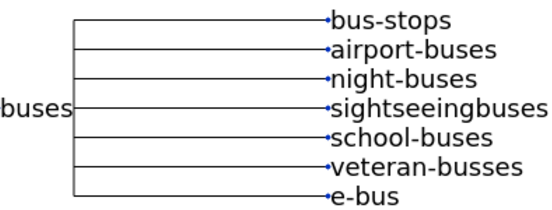
\includegraphics[width=0.5\textwidth]{buses-cat-tree}
        \caption{\textit{buses} category sub-tree of the NTB category tree}
        \label{fig:buses-cat-tree}
    \end{figure}
    
    
    % * wordnet types included
    % * extending parent category with additional images and including parent label itself
    
    % types of categories (maybe according to wordnet):
    % \begin{itemize}
    %     \item actions: swimming, fighting with fire
    %     \item objects: 
    %     \item
    % \end{itemize}
    
    
    % Some pictures were labeled with parents label, in most cases such labels were removed since it is usually not a good idea to mix children (e.g. colors).
    
    % If selected category (the one that satisfies all criteria) had also children categories which were subcategories of the parent one then pictures labeled with such children categories were also included in the parent category, even if child category by itself was not included in the final selection. For example, buses: school-buses, night-buses, bus-stops (maybe cars example is better). In this example images labeled with school-buses and night-buses (but not bus-stops) will be included in the buses category since there subclass relationship is taking place, even though night-buses doesn't satisfy criteria and thus will not be included in the final selection. This was made to both keep granularity of children categories, and to use information from the parent labels since in some cases parent label contained more pictures than all its descendants combined, more example of such parent categories: flowers, trees and dogs.
    
    
    % context-dependent image vs context-dependent term
    
    % Exceptions: no-people
    % Double meaning examples: newsparers (companies and actuall newspapers)
    
    
    
    
    % examples of relationships:
    % \begin{itemize}
    %     \item Subclass: buses -> school-buses
    %     \item Part-of: hands -> fingers
    % \end{itemize}
    
    % YES: dogs: types, NO: fruit: types
    
    % non-subclass relationship: tram -> tram-stop
    
    \subsection{Dataset preparation}
    Using the categories tree, described in the previous section, a base dataset was created. Figure \ref{fig:main-cat-num-vs-threshold} shows the number of categories with an amount of images above the specified threshold. It is clearly visible that the majority of categories has a low number of images. For example, more than half of the categories contain less than 50 images.
    
    
    \begin{figure}[h!]
        \centering
        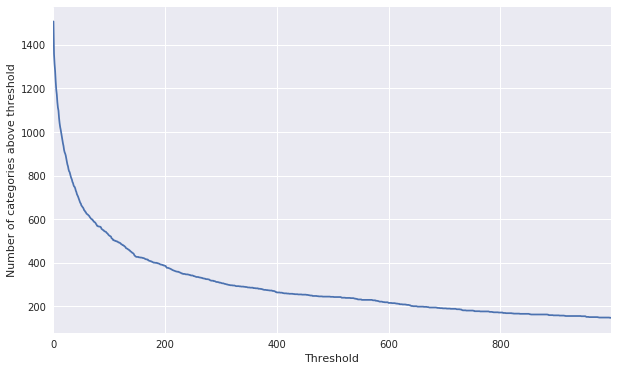
\includegraphics[width=\textwidth]{main-cat-num-vs-threshold}
        \caption{Number of categories with amount of images above particular threshold}
        \label{fig:main-cat-num-vs-threshold}
    \end{figure}
    
    Due to the big number of categories and the multi-label case of classification, which makes it challenging to find particular threshold value that will suit the purpose, it was decided not to perform balancing of the dataset in the main experiment. One of the reasons why finding appropriate threshold can be a challenging task, in this case, is that some categories can be tightly connected and therefore removal images from one of them can also affect the number of images in other categories. Additionally, it was considered challenging to choose a single, justified value of a threshold for the purpose of the experiment.
    
    A new method of splitting the dataset into training, validation and test sets was used. Instead of performing split on a per-category basis like in the trial experiments, the whole set of images was created and randomly split into three parts with the specified ratio (60\%/20\%/20\%). This method gives better average split on the subset for a multi-label case, as it is shown in the results section \ref{sec:split-comparison}. As it was discussed in the section \ref{sec:trial-dataset-prep} of a trial experiment, there is a challenge of splitting multi-label dataset, especially with the high level of coherency between categories. Since the splitting process is random and in order to satisfy the requirement of having a minimum number of one image for each category in each of the three sets, it was empirically discovered that the minimum number of images in each category should be 50 for the given dataset. Therefore all categories below this threshold were removed living 663 categories in the final dataset. In order to be able to compare results of different implementations, one image dataset was created and then used in the training, in contrast to the trial experiments where dataset, as well as training, validation and test split were random for each training process. This was achieved by setting random seed in the beginning of the splitting process and by reusing created LMDB files.
    
    % No balancing of the dataset was performed due to number of reasons: big number of categories and multi-label case of classification makes it hard to find  big difference in the number of images between categories and due to big number of categories. Considering this, it was hard to find particular threshold which could be used 
    
    
    \subsection{Training process}
    Mostly the same training process described in the section \ref{sec:trial-training} was used in the main experiments, all differences in the process are described in this section. 
    
    Due to a new hardware available during the main experiment phase, in addition to CaffeNet classification system was trained on the newer GoogleNet DNN \cite{Szegedy2015GoingDeeper}. The same fine-tuning approach was applied. The CaffeNet was adapted to a multi-label case in the same way as during trial experiment.
    
    Since GoogleNet introduced new InceptionLayer, which combines an output of the three fully connected layers on the last levels of the network, in addition to DataLayer all these three layers had to be replaced with new ones in order to train network to classify the new set of categories. Each of this three layers has their own loss layer which was also replaced by a SigmoidCrossEntropyLoss layer. For the same reason as in CaffeNet, all three Accuracy layers were removed from the network.
    
    Adam solver algorithm was used since it showed much better result compared to Stochastic Gradient Descent during the trial experiment.

    The usage of LMDB as an image data source showed good results during the trial experiments, therefore it was decided to adapt this solution to the multi-label case. While in single-label case image label is a number that identifies to which category this image belongs to, in multi-label case label data have to be a vector of numbers or binary vector where value 1 on the $i$th position indicates that image belongs to the category $i$. In order to do that, two LMDB files were created: one for image data only, and one for labels which are represented as a ground-truth two-dimensional matrix.  
    
    Since new GPU had more memory (12GB vs 3GB on old one), batch size for CaffeNet was increased to 900 during the training phase and to 200 during the validation phase, corresponding values of 128 and 16 were used for training of GoogleNet. The same hyper-parameters as during the trial experiment with Adam solver were used for training, except that test iterations were chosen to cover the whole validation set of images: 700 and 8600 for CaffeNet and GoogleNet correspondingly.
    
    In contrast to trial experiments, during the main experiments training process was stopped after a loss on the validation set was stabilized in order to get the most from the used dataset and network and to avoid overfitting.

    \subsection{Testing process}
    The same testing process was used as during the trial experiment described in the section \ref{sec:trial-testing}.
    
    Similar to the adaptation of the deployment version of CaffeNet, DataLayer of the deployment version of GoogleNet was replaced with the Input layer with the corresponding dimensions. Only one from three fully connected layers are presented in the final version of GoogleNet specification, therefore only this layer was changed to the newly trained layer and its corresponding loss layer was replaced with the Sigmoid layer.
    
    \subsection{Hardware}
    \label{sec:main-hw}
    \begin{itemize}
        \item \textbf{CPU} -- Intel(R) Xeon(R) CPU E5-1620 v4 @ 3.50GHz
        \item \textbf{GPU} -- NVIDIA Titan X Pascal
        \item \textbf{RAM} -- 32 GB
        \item \textbf{Storage} -- SK hynix SC308 256 SSD
    \end{itemize}

    
\section{Libraries and tools}
This section gives description of used libraries and tools in experiments as well as motivation for using them.

\begin{itemize}
    \item \textbf{Caffe} \cite{Caffe} is a one of the most widely adopted in the industry deep learning framework. In addition to the training framework itself it provides with collection of pretrained models from different research papers \cite{CaffeModelZoo} and Python language bindings. It also allows to run training on the CUDA \cite{CUDA} enabled graphics cards which significantly improves both training and testing speed \cite{Krizhevsky2012ImageNetDNN}.
    \item \textbf{NumPy} \cite{numpy} is a Python library for scientific computing. This library was used in the project for computations optimization trough vectorized calculations.
    \item \textbf{pandas} \cite{pandas} is a Python library which provides efficient data manipulation trough different datastructures as well as its visualization. It was used for tables representations and drawing charts.
    \item \textbf{Jupyter Notebook} \cite{jupyter} is a web application for live coding, visualization, numerical simulation etc. This application was used for both remote code editing and tables/charts visualizations.
    \item \textbf{ETE Toolkit} \cite{ete3} is a Python framework for tree visualization and analysis. It was used for categories tree parsing (using newick \cite{newick} format), processing and visualization.
    \item \textbf{vagga} \cite{vagga} is a tool that helps to describe and build development environment as well as to run processes inside of it. It also provides different levels of process isolation through Linux namespaces \cite{namespaces} kernel feature. It was used to specify the whole research project environment. Isolation properties that it gives as well as full declarative system specification should improve project reproducibility.
\end{itemize}
